\subsection{Задача распознавания диктора}

Распознавание диктора является одной из задач обработки речи --- обширного
научного-исследовательского направления с долгой и богатой историей. Как и в
случае со многими другими научными направлениеями, в последние годы обработка
речи стала активно использовать методы машинного обучения, в частности
нейросетевые модели. Так, впечатляющих результатов удалось добиться не только в
распознавании диктора~\cite{xvectorspaper,sincnet}, но и в смежных областях
автоматического распознавания~\cite{wav2vec2} и синтеза речи~\cite{tacotron2}.

Задача распознавания диктора, как нетрудно понять из названия, заключается в
определении личности человека по аудиозаписи его речи. Если говорить чуть
более строго, задачей является сопоставление некоторой аудиозаписи речи
неизвестного человека с некоторым набором дикторов. В случае решения задачи
\emph{идентификации} этот набор состоит из нескольких дикторов, при этом мы
точно знаем, что один из них произнес анализируемую нами речь. Соответственно,
в таком случае задачей системы является правильный выбор диктора. В случае
решения задачи \emph{верификации} нам известна информация только об одном
дикторе, и от нас требуется определить, произнёс ли он речь на предоставленной
аудиозаписи.

Может показаться, что две указанные проблемы существенно отличаются и,
соответственно, требуют для своего решения различные системы. На самом деле,
это не так. Задача распознавания диктора в общем случае может быть
представлена~\cite{sr_chapter} как сравнение модели диктора и вектора признаков
анализируемой речи. Тогда каждой паре диктор--аудио можно сопоставить некоторое
число, характеризующее степень соответствия. При идентификации мы получим
несколько чисел, наибольшее из которых будет указывать на наиболее вероятного
диктора. При верификации нам нужно будет просто преобразовать единственное
полученное число в вероятность. Если говорить в терминах глубокого обучения,
отличаться будет только последняя функция активации: при идентификации это будет
$\softmax$, при верификации --- $\sigmoid$.

В целом модель диктора может принимать различные формы. Например, в течение
продолжительного времени одним из ведущих методов моделирования дикторов
была~\cite{sr_chapter} модель смеси гауссиан (\textit{Gaussian Mixture Model}).
В современных нейросетевых системах модель диктора обычно представляет собой
вектор признаков. Тогда задача определения степени соответствия диктора и речи
сводится к сравнению двух векторов, которое можно осуществлять как с помощью
вычисления косинусного расстояния, так и с использованием более сложных методов
--- вероятностного линейного дискриминантного анализа (\textit{Probabilistic
Linear Discriminant Analysis})~\cite{PLDA} или нейронных сетей~\cite{Zeng_2022}.
В оригинальной статье~\citeisr{}, посвященной исследуемому в этой работе методу,
нейронные сети используются как для моделирования диктора, так и для расчёта
метрики соответствия диктора и речи.  Мы будем придерживаться такого же подхода.

\subsection{Общие принципы метода}\label{ssec:isr}

На рис.~\ref{fig:isr} проиллюстрирован метод интерактивного распознавания
диктора. Изначально у нас имеется $K$ дикторов, далее мы случайно выбираем из
них одного целевого --- его модуль распознавания диктора (\textit{SR Module}) и
будет пытаться угадать. Как уже было сказано ранее, каждый диктор
характеризуется своим вектором признаков (эмбеддингом диктора или \textit{voice
print} --- голосовой подписью). Данные о дикторах передаются модулю
распознавания диктора, после чего он выбирает, какое слово должен произнести
угадываемый диктор. Диктор произносит это слово, новая аудиозапись поступает на
вход SR-модуля, и он запрашивает новое слово.  Процесс повторяется, пока
SR-модуль не получает $T$ аудиозаписей слов, после чего он пытается угадать
целевого диктора.

\begin{figure}[hbt]
    \centering
    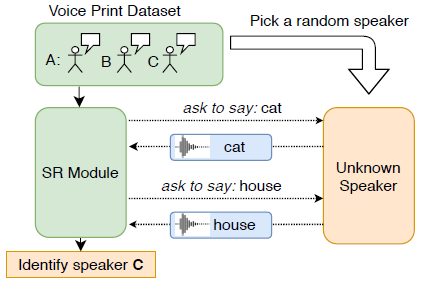
\includegraphics[scale=1.0]{figures/isr_game.png}
    \caption{Схема интерактивной игры по определению диктора \citeisr.}
    \label{fig:isr}
\end{figure}

Стоит отметить несколько важных моментов рассматриваемого метода:
\begin{enumerate}
    \item Выше был описана задача идентификации. В этой работе мы тоже будем в
    основном решать именно eё, хотя с практической точки зрения нам интереснее
    верификация. Такое решение объясняется двумя причинами.  Во-первых, задача
    идентификации является более гибкой --- варьиюруя число дикторов $K$ её
    можно делать более или менее сложной. Во-вторых, как будет
    продемонстрировано в разделе~\ref{ssec:verification}, перейти от
    идентификации к верификации достаточно просто.
    \item Все векторы признаков дикторов и произнесенных слов вычисляются с
    помощью отдельной нейронной сети, более подробное описание будет дано в
    разделе~\ref{ssec:data}. Далее мы будем обычно говорить не об аудиозаписях,
    а об эмбеддингах дикторов и слов, которые и будут получать на вход
    нейросетевые модели для распознавания диктора.
    \item Две функции SR модуля --- идентификация диктора и выбор запрашиваемых
    слов --- выполняют две различные нейронные сети. Такое разделение вовсе не
    является обязательным, но оно позволяет использовать обучение с учителем для
    нейросети, решающую задачу идентификации.
\end{enumerate}

\subsection{Нейросетевые модели --- \guesser{} и \enquirer{}}\label{ssec:nnet}

Итак, рассмотрим внутреннее устройство модуля для распознавания диктора. В
первую очередь стоит изучить модель, решающую непосредственно задачу
идентификации, которую авторы~\citeisr{} назвали \guesser{}. Её архитектура
(рис.~\ref{fig:guesser}) достаточно проста. Сначала эмбеддинги дикторов $g_i$
усредняются, полученный вектор $\hat{g}$ подаётся в качестве запроса в блок
с механизмом внимания (\textit{Attention Layer}).

\begin{figure}[hbt]
    \centering
    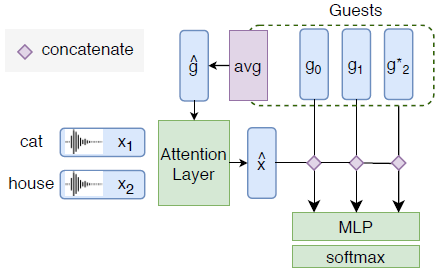
\includegraphics[scale=1.0]{figures/guesser.png}
    \caption{Архитектура нейросети \guesser{}~\citeisr.}
    \label{fig:guesser}
\end{figure}

Другие входные данные --- эмбеддинги произнесённых диктором слов $x_i$ ---
используются в Attention слое в качестве ключей и значений. В~\citeisr{}
приведены следующие формулы для расчёта вектора $\hat{x}$:
\begin{equation*}
    e_t = \text{MLP}([x_t, \hat{g}]); \quad \alpha = \text{softmax}(e); \quad
    \hat{x} = \sum_t{\alpha_t x_t};
\end{equation*}
где $\text{MLP}$ --- многослойный перцептрон, a $[.,.]$ --- операция
конкатенации. Как мы видим, в данном случае используется аддитивная версия
механизма внимания.

Далее вектор $\hat{x}$ конкатенируется к каждому эмбеддингу диктора $g_i$,
результат пропускается через многослойный перцептрон, рассчитывающий метрику
соответствия. Для превращения этих $K$ чисел в вероятностное распределение
используется операция $\softmax$.

Здесь и далее многослойный перцептрон имеет 1 скрытый слой, использует в
качестве функции активации ReLU, а также применяет на скрытом слое операцию
Dropout с $p=0.5$.

\begin{figure}[hbt]
    \centering
    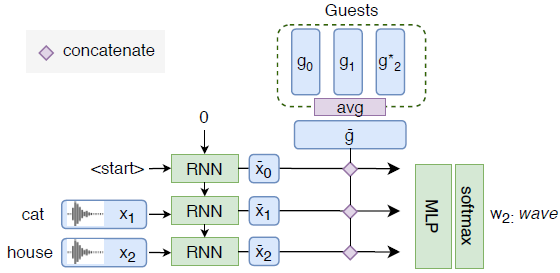
\includegraphics[scale=1.0]{figures/enquirer.png}
    \caption{Архитектура нейросети \enquirer{}~\citeisr.}
    \label{fig:enquirer}
\end{figure}

Архитектура нейросети \enquirer{} (рис.~\ref{fig:enquirer}), выполняющей
функцию выбора запрашиваемого слова, тоже относительно проста. В ней для
аггрегации информации о запрошенных (и услышанных) ранее словах используется
рекуррентная нейронная сеть (\textit{RNN}), если быть точнее --- BiLSTM\@.
Далее к последнему скрытому состоянию BiLSTM конкатенируется усреднённый
эмбеддинг дикторов, результат пропускается через MLP. Выходная размерность
равна $V$ --- числу слов в словаре.

\subsection{Мотивация}\label{ssec:ytho}

Теперь, когда мы разобрались с устройством предлагаемой системы распознавания
диктора, возникает логичный вопрос --- есть ли у неё какие-либо преимущества
относительно существующих решений? И какую цель преследует добавление модели для
выбора запрашиваемых слов?

В оригинальной работе~\citeisr{} основная идея --- адаптация системы под
идентифицируемых в данный момент дикторов. Различия в произношении могут
объясняться как акцентом человека, так и его индивидуальными особенностями.
Поэтому важные признаки будут отличаться от диктора к диктора, соответственно,
для наиболее быстрого распознавания будут требоваться различные слова. Таким
образом, главное преимущество предлагаемого подхода --- распознавание диктора с
использованием минимального количества тестовых аудиозаписей речи.

Стоит отметить, что сегодня уже существуют решения\footnote{
    Здесь сошлёмся на экспертные знания сотрудников лаборатории Huawei CBG AI
}, позволяющие надёжно верифицировать пользователя по очень коротким
аудиозаписям. Проблема этих решений заключается в том, что человек должен
произнести некоторые слова из ограниченного списка. Это создаёт риск т.~н.
спуфинга --- злоумышленник может обмануть систему, предоставив ей запись речи
верифицируемого человека. Хотя оригинальная имплементация разрабатываемой
системы едва ли решает эту проблему --- выбор осуществляется из фиксированного
списка из 20 слов, нейросеть для выбора запрашиваемых слов может быть изменена
таким образом, чтобы исправить этот недочёт (см. главу~\ref{ssec:codebook}).

\subsection{Выводы и результаты по главе}

\begin{itemize}
    \item Задача распознавания диктора (\textit{speaker recognition}) активно
    изучается в течение многих лет и представляет большой практический интерес.
    \item В ряде случаев система распознавания диктора может выбирать, какую
    фразу произнесет пользователь. В таком случае логично использовать алгоритм,
    позволяющий за счёт выбора фраз сократить количество запрашиваемой речи и/или
    увеличить точность распознавания.
    \item В качестве такого алгоритма можно использовать предложенную в \citeisr{}
    нейросетевую модель.
\end{itemize}